%%
%  ******************************************************************************
%  * #file    Szablon_raportu_EN_Latex.tex
%  * #author  Adrian Wójcik   adrian.wojcik(at)put.poznan.pl
%  *          
%  * #commit  Patryk Kościk   koscikpatryk(at)gmail.com
%  *          Modified the template for Projekt przejsciowy purposes          
%  *          
%  * #version 1.0
%  * #date    09-Mar-2022
%  * #brief   PROJPRZEJ
%  *
%  ******************************************************************************
%%  
\documentclass[11pt, a4paper]{article}

\usepackage{SM_template}

% Wypełnijcie te dyrektywy zgodnie z waszym tematem
% \lab      -> NAZWA CZUJNIKA, np.: 'DHT22'
% \comment  -> Króciutki opis co to, np.: 'Cyfrowy budżetowy czujnik temperatury'
%

\lab{Moduł KY-004}
\comment{Analogowy przełącznik mechaniczny monostabilny}
\author{Dawid Wasung}
\addbibresource{bib/KY-004.bib}

% Absolutny zakaz dotykania tego tutaj bo jak dotkiecie to coś jebnie
\university{Politechnika Poznańska}
\faculty{Wydział Automatyki, Robotyki i Elektrotechniki}
\institute{Instytut Robotyki i Inteligencji Maszynowej}
\department{Zakład Sterowania i Elektroniki Przemysłowej}

\nocite{*}


%%
%
% Początek dokumentu
%
%%
\begin{document}

%% Strona tytułowa %%
\mainpage{{KY-004/przycisk}}
\newpage

\section*{Opis elementu} \addcontentsline{toc}{section}{Wstęp}
Czujnik KY-004 składa się z przycisku monostabilnego, wbudowanego rezystora 10k $\Omega$ oraz trzech pinów męskich. Sam przycisk jest ręcznym łącznikiem elektrycznym niskiego napięcia. Powraca on do swojej pozycji po usunięciu siły zewnętrznej (lub po odblokowaniu), która najczęściej ma załączyć lub rozłączyć dany obwód. 
\vspace{0.5cm}
\begin{figure}[h]
\centering
\begin{subfigure}{.5\textwidth}
  \centering
  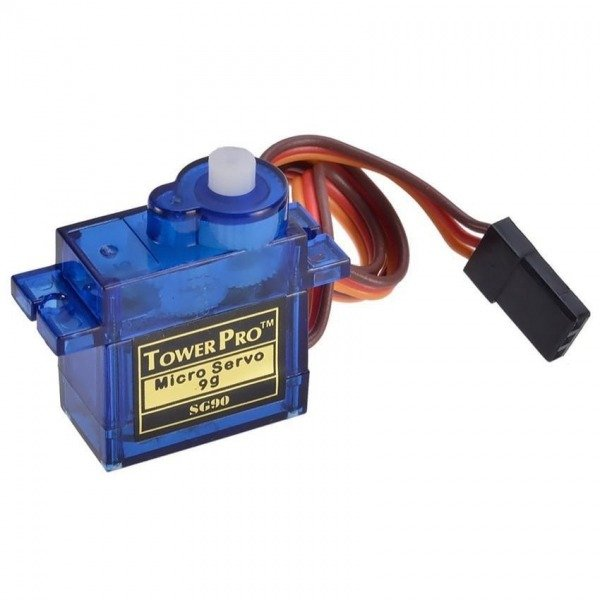
\includegraphics[width=.4\linewidth]{fig/KY-004/zdj_modułu/fig1.png}
  \caption{Moduł KY-004 \cite{ArduinoModules:Switch}}
  \label{fig:sub1}
\end{subfigure}%
\begin{subfigure}{.5\textwidth}
  \centering
  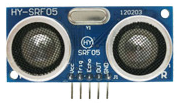
\includegraphics[width=0.95\linewidth]{fig/KY-004/zdj_modułu/fig2.png}
  \caption{Przycisk monostabilny (THT) \cite{ArduinoModules:grab}}
  \label{fig:sub2}
\end{subfigure}
\caption{Poglądowe rysunki modułu oraz przycisku}
\label{fig:test}
\end{figure}
\vspace{0.5cm}

Przycisk jest elementem kontrolującym przepływ prądu w obwodzie - kluczową rolę odgrywają w układach, w których potrzebna jest interakcja użytkownika. Mogą znajdować się w dwóch stanach: otwartym (przerwa w obwodzie; występuje w przypadku braku interakcji z przyciskiem lub po jego puszczeniu - wyłączony) oraz zamkniętym (obwód zamknięty, przycisk działa jak rzeczywisty przewodnik; występuje w przypadku, gdy przycisk jest wciśnięty - włączony). 

\vspace{0.5cm}
\begin{figure}[h]
\centering
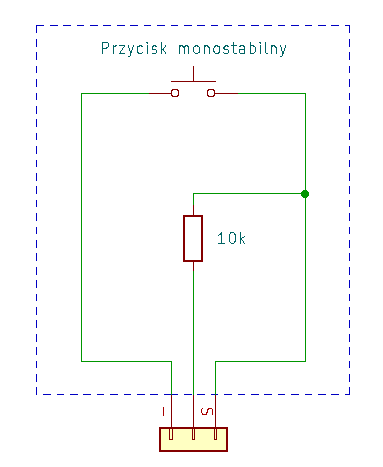
\includegraphics[width=.4\linewidth]{fig/KY-004/zasada_dzialania/schemacik.png}
\caption{Schemat modułu}
\label{fig:sub2}
\end{figure}
\vspace{0.5cm}



\section*{Użycie czujnika}
Przycisk ze względu na swoje działanie oraz prostotę implementacji jest jednym z najpowszechniej używanych elementów w fizycznych układach elektrycznych - użytkownik odpowiedzialny jest za jedną akcję, reszta dzieje się automatycznie. Używa się go wszędzie tam, gdzie wymagane do sterowania jest użycie impulsu, przykładowo w urządzeniach konsumenckich czy zastosowaniach przemysłowych.


Poniżej przedstawiono podstawową implementację czujnika na płytce stykowej - wciśnięcie przysiku załącza diodę LED.

\vspace{0.5cm}
\begin{figure}[h!]
    \centering
    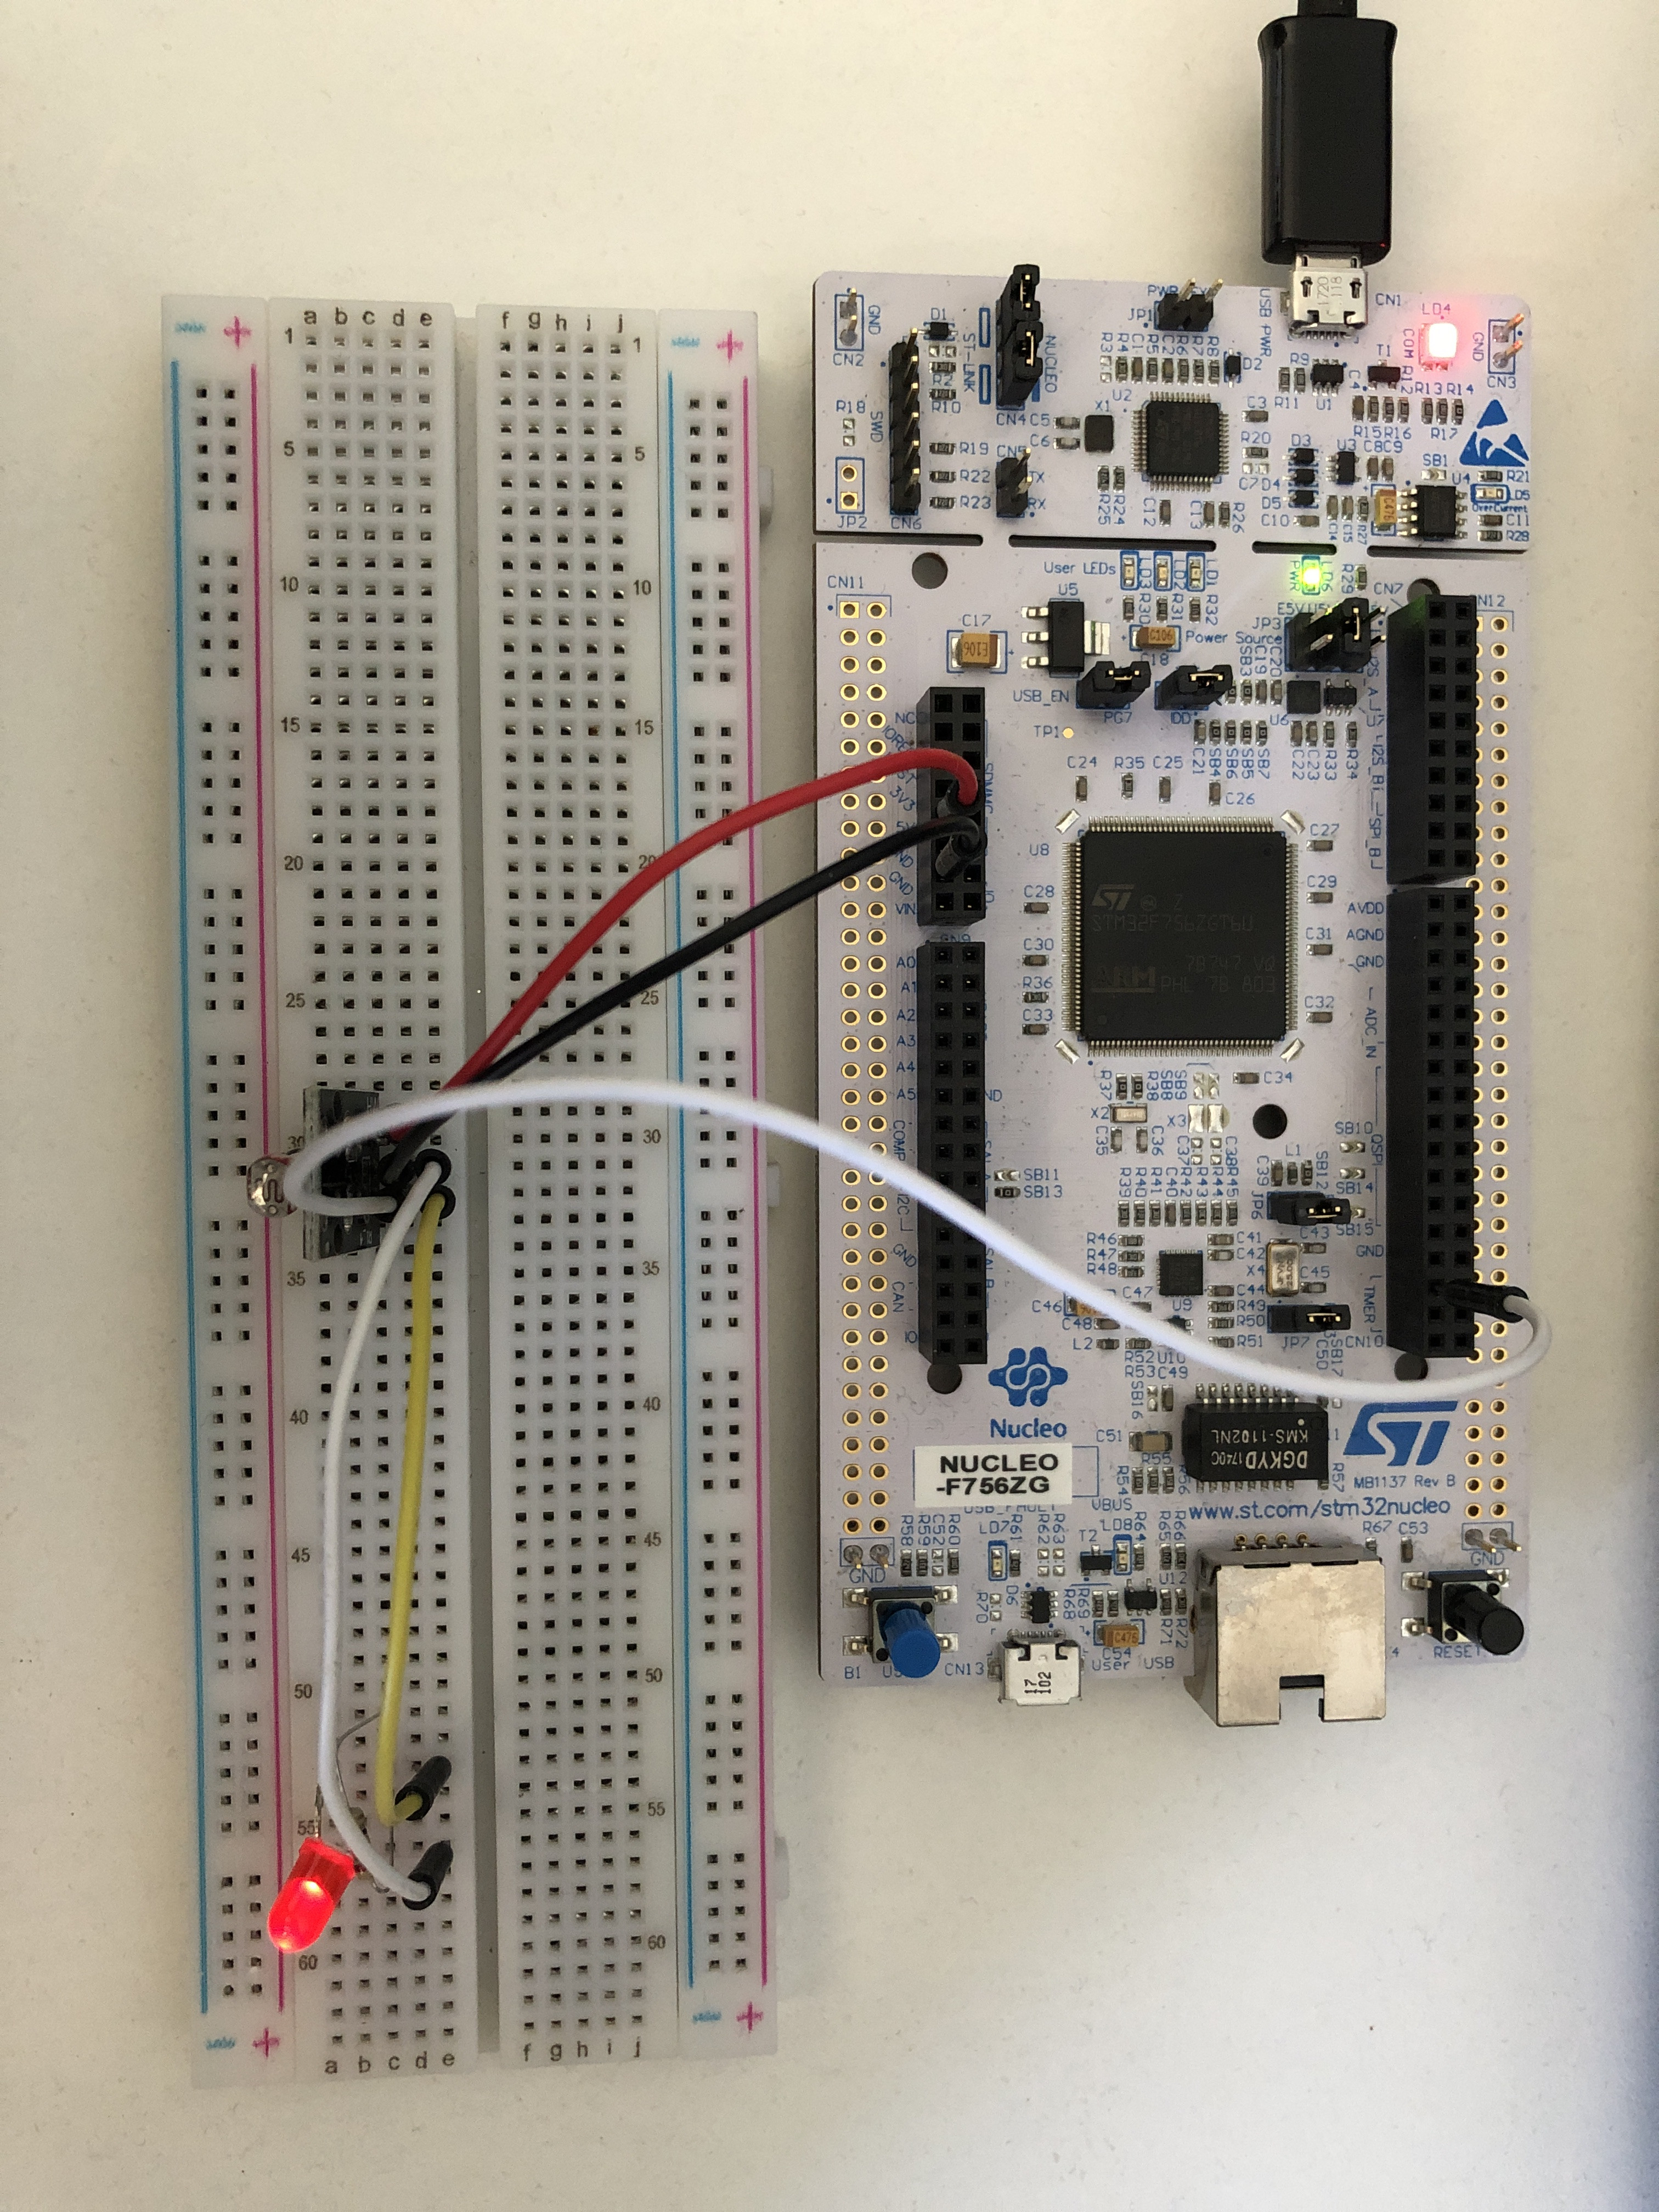
\includegraphics[width=0.6\textwidth]{fig/KY-004/działanie_ukladu/final.jpg}
    \caption{Przycisk wyłączony}
    \label{fig:my_label}
\end{figure}

Na Rys.3 widnieje zbudowany układ z modułem KY-004. Przycisk jest wyłączony, użytkownik nie wchodzi z nim w interakcje - oobwód jest przerwany, prąd przez diodę nie płynie i przez to nie świeci.

\vspace{0.5cm}

\begin{figure}[h!]
    \centering
    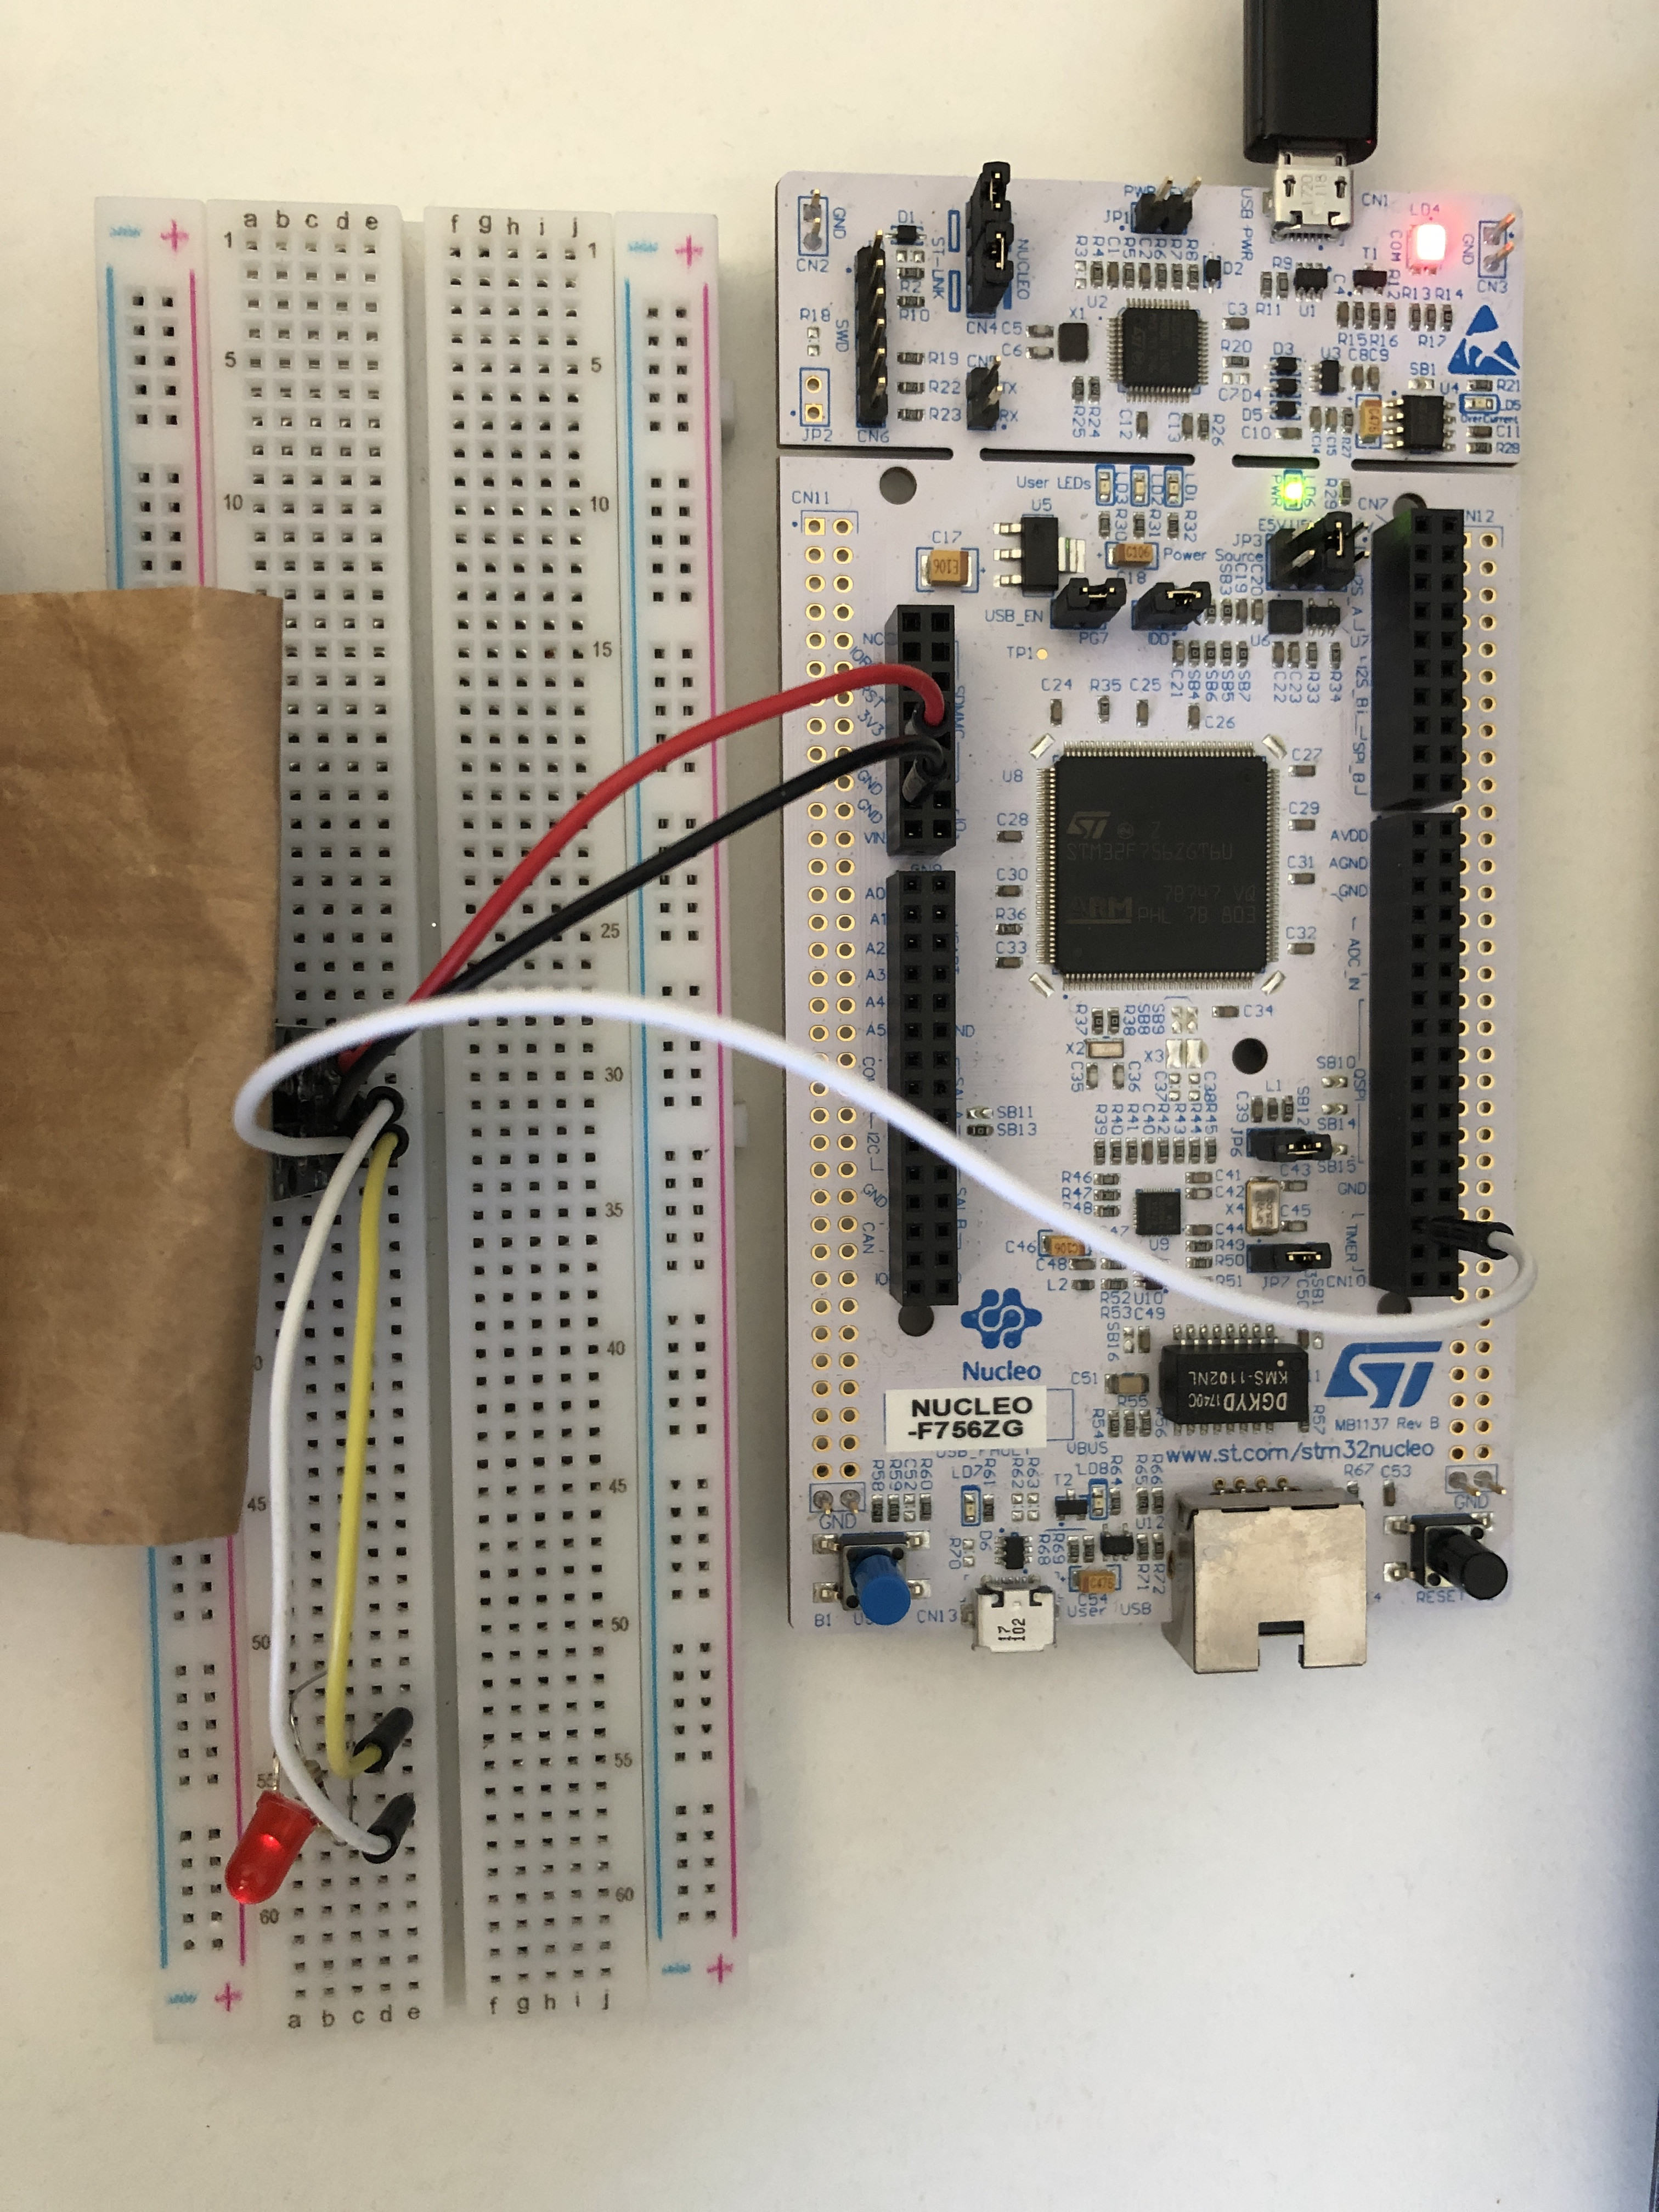
\includegraphics[width=0.6\textwidth]{fig/KY-004/działanie_ukladu/final2.jpg}
    \caption{Przycisk włączony}
    \label{fig:my_label}
\end{figure}

Na Rys.4 użytkownik wciska przycisk - jest wyłączony, styki się zwierają i obwód się zamyka; prąd zaczyna płynąć przez diodę na płytce stykowej, co powoduje jej świecenie. Można również zauważyć zmianę stanu diody na płytce Nucleo spowodowaną wykryciem zbocza. 
\newline 



Kod programujący czujnik, wykorzystany do opracowania instrukcji, znajduje się w materiałach dodatkowych zawartych pod koniec rozdziału.
\newline
Film prezentujący działanie układu znajduje się w suplemencie wideo.
\printbibliography[heading=bibintoc]

\end{document}